\documentclass[10pt, preprint]{aastex}

\usepackage{natbib}
\bibliographystyle{plainnat}

\usepackage{minted}
\usepackage{float}
\usepackage{graphicx}
\usepackage{subfig}
\usepackage{amsmath}
\usepackage[toc,page]{appendix}
\usepackage[utf8]{inputenc}
\usepackage{hyperref}
\usepackage{url}
\hypersetup{
    colorlinks=true,
    linkcolor=blue,
    filecolor=magenta,      
    urlcolor=blue,
    citecolor=blue,
}
\usepackage{booktabs}
\renewcommand{\arraystretch}{1}

\title{CTA200 Assignment \#3}

\author{Madeline Nardin}

\begin{document}

\section{Question 1}
The first part of this assignment involved iterating over a complex grid, and plotting the bounded and divergent solutions in two different manners. A grid of complex points was formed with the constraints $-2<x<2$ and $-2<y<2$, using the \texttt{numpy.outer()} function, to create a 20x20 matrix of real and a second 20x20 matrix of complex points. The sum of these two matrices was then computed to obtain a grid of complex numbers within the desired constraints. Next each point within the grid was inputted into the function \texttt{iterate.py}, which iterates the equation shown in equation \ref{eq:iterate} with a maximum of 10 iterations.
\begin{equation}\label{eq:iterate}
    z_{i+1} = z_i^2 +c \; \mbox{ such that } c = x + iy
\end{equation}
The function then computes the absolute length given in equation \ref{eq:length}, and categorizes whether the point remains bounded under the condition that $|z|<=2$, otherwise the point diverges. The function then returns the points which remain bounded and the points which diverge and the number of iterations at which the point diverges.
\begin{equation}\label{eq:length}
    |z|^2 = \Re(z)^2 + \Im(z)^2
\end{equation}
Figure \ref{fig:q1a} displays the points that diverge under these conditions in red and the points which remain bounded in blue plotted on the complex plane and Figure \ref{fig:q1b} displays the points that diverge on the complex plane with a color bar indicating the iteration number at which the given point diverged.
\begin{figure}[H]
  \centering
  \subfloat[]
  {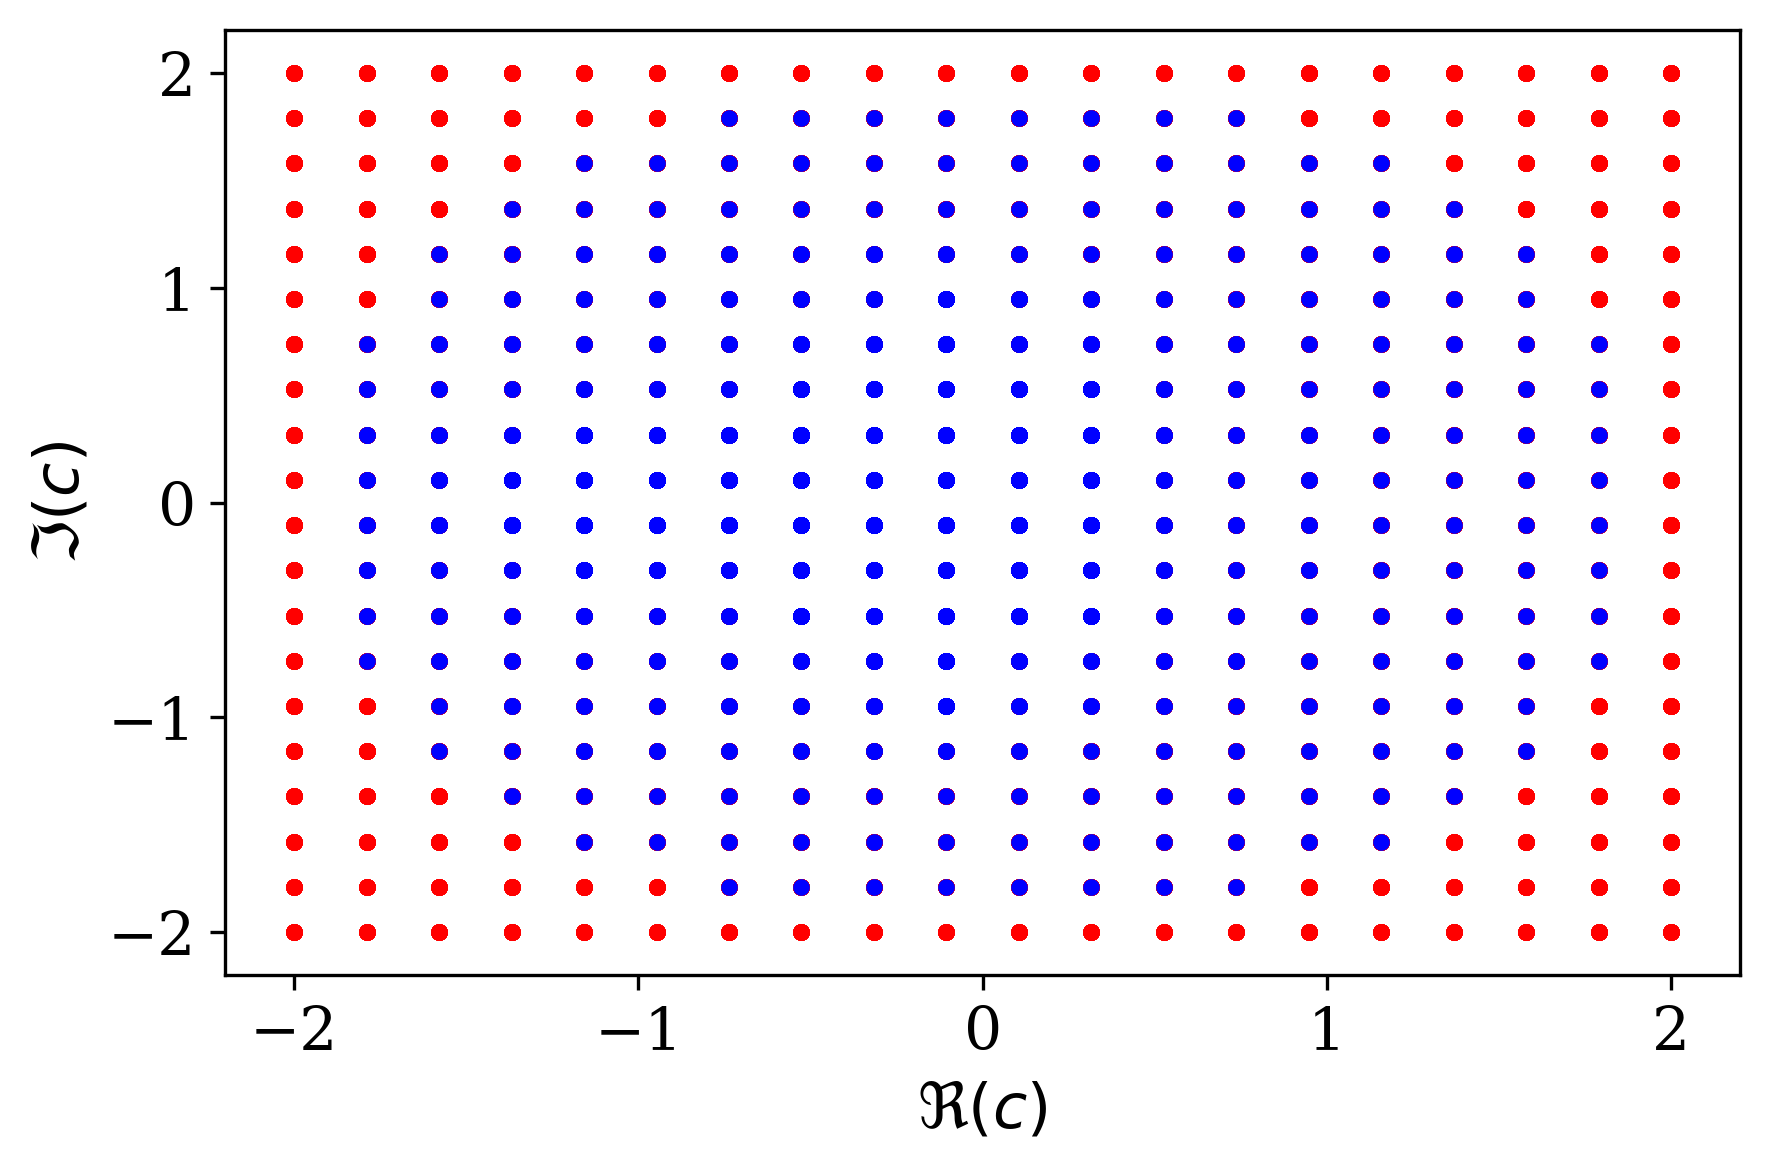
\includegraphics[width = 0.49\textwidth, height = 0.35\textwidth]{q1.png}\label{fig:q1a}}
  \hfill
  \subfloat[]{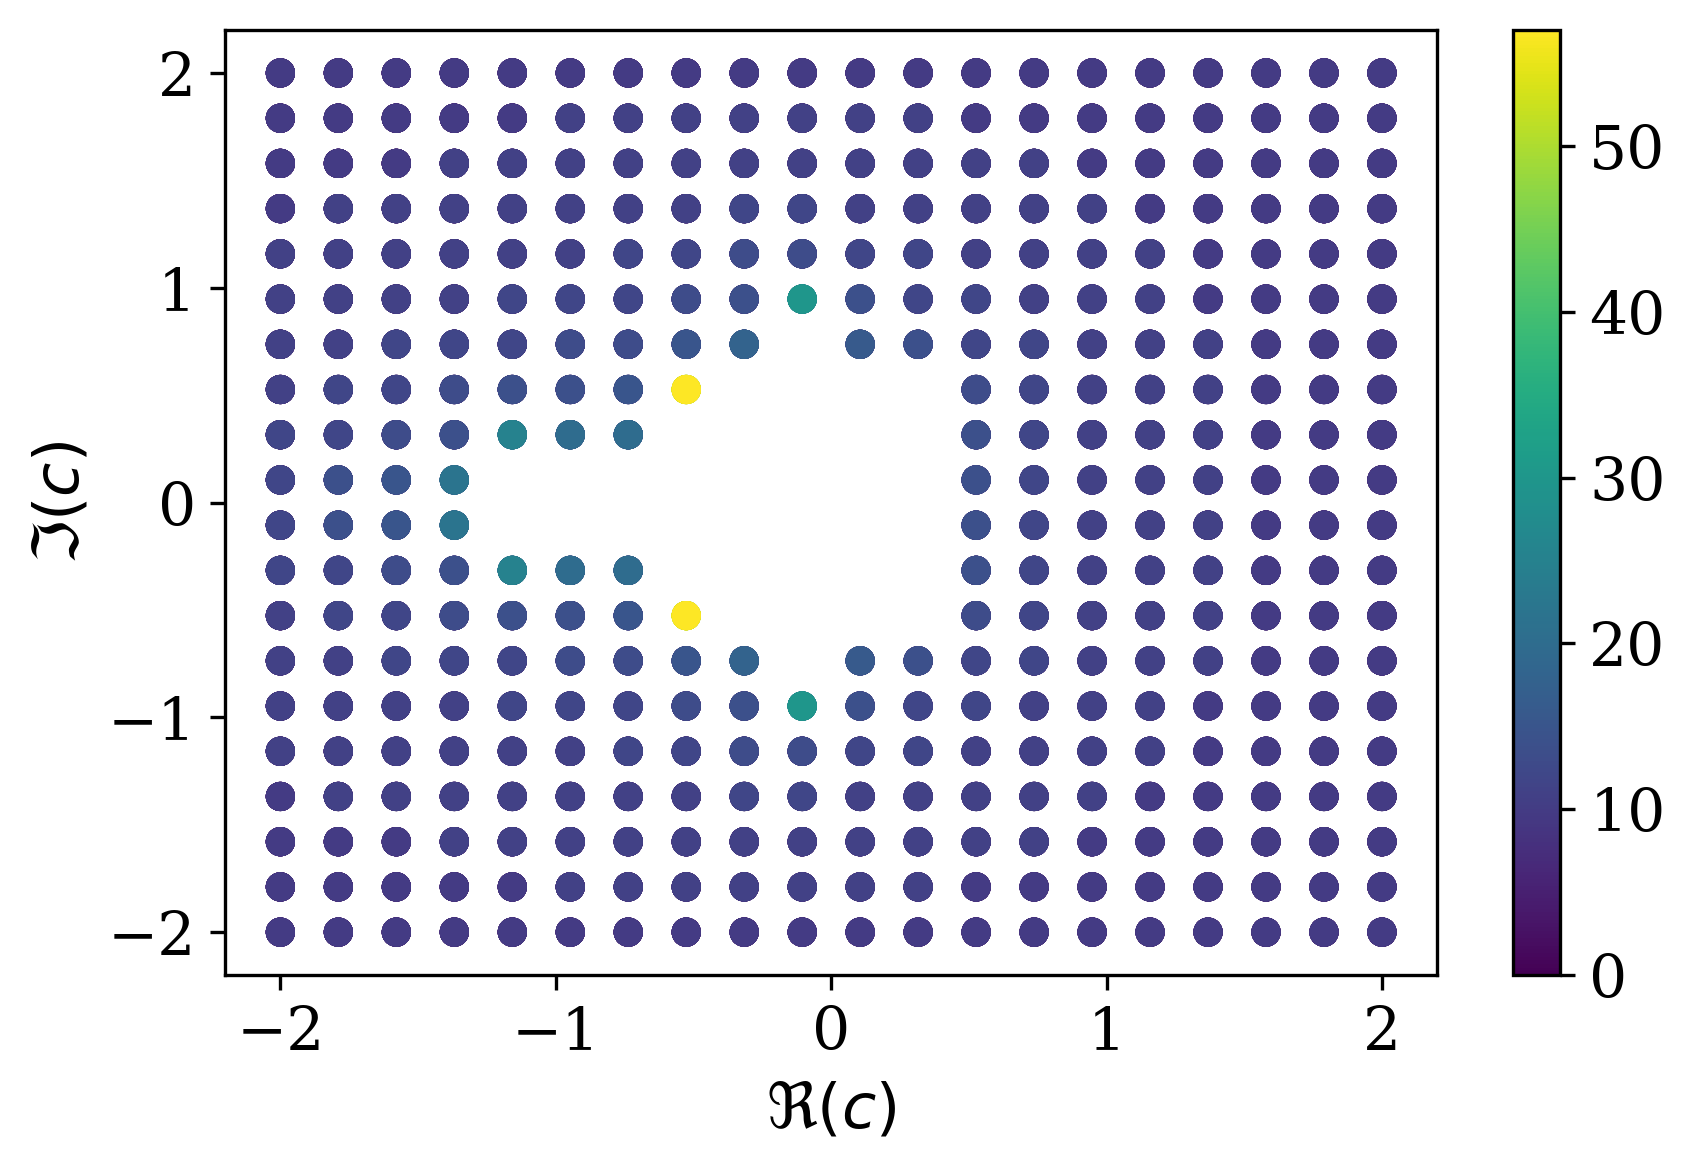
\includegraphics[width = 0.49\textwidth, height = 0.35\textwidth]{q1cbar.png}\label{fig:q1b}}
    \hfill
  \caption{ Bounded points (blue) and divergent points (red) plotted on the complex plane (a) and divergent points with iteration number color bar (b) for all points within a complex grid defined by $-2<x<2$ and $-2<y<2$. \label{fig:q1}}
\end{figure}

\section{Question 2}
The second part of this assignment involved recreating the results found in \cite{Lorenz} by modeling the behavior of the atmosphere. \cite{Lorenz} defines the three equations shown below.
\begin{equation}\label{eq:x}
    \dot{X} = -\sigma(X-Y)
\end{equation}
\begin{equation}\label{eq:y}
    \dot{Y} = rX - Y - XZ
\end{equation}
\begin{equation}\label{eq:z}
    \dot{Z} = -bZ +XY
\end{equation}
Equations \ref{eq:x}, \ref{eq:y} \& \ref{eq:z} involve three dimensionless parameters: $\sigma$ denotes the Prandtl number, r denotes the Rayleigh number and b is a length scale. Equations \ref{eq:x}, \ref{eq:y} \& \ref{eq:z} were solved with the initial condition $W_0 = [0.0,1.0,1.0]$ and parameters $[\sigma,r,b] = [10.0,28.0,8.0/3.0]$ with \texttt{scipy.integrate.solve\_ivp} over $0\le t \le60$. Figures 1 \& 2 from \cite{Lorenz}, were then recreated and are displayed in Figure \ref{fig:q2}. 

\begin{figure}[H]
  \centering
  \subfloat[]
  {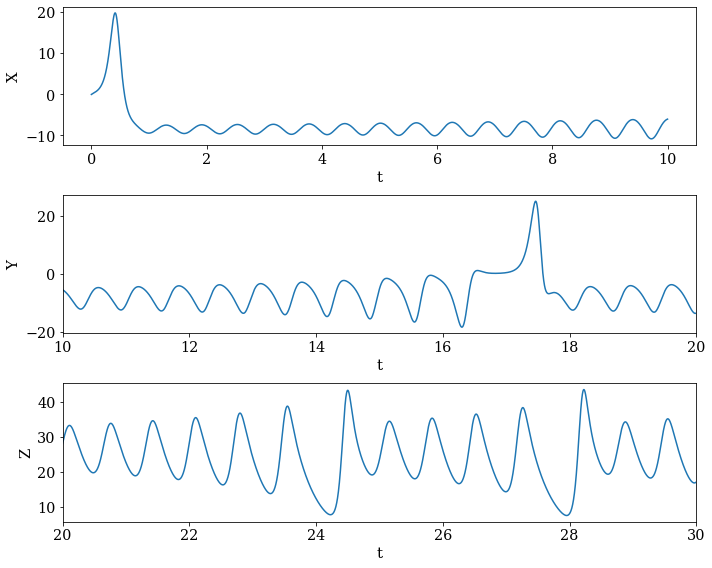
\includegraphics[width = 0.49\textwidth, height = 0.35\textwidth]{q2fig1.png}\label{fig:q2fig1a}}
  \hfill
  \subfloat[]{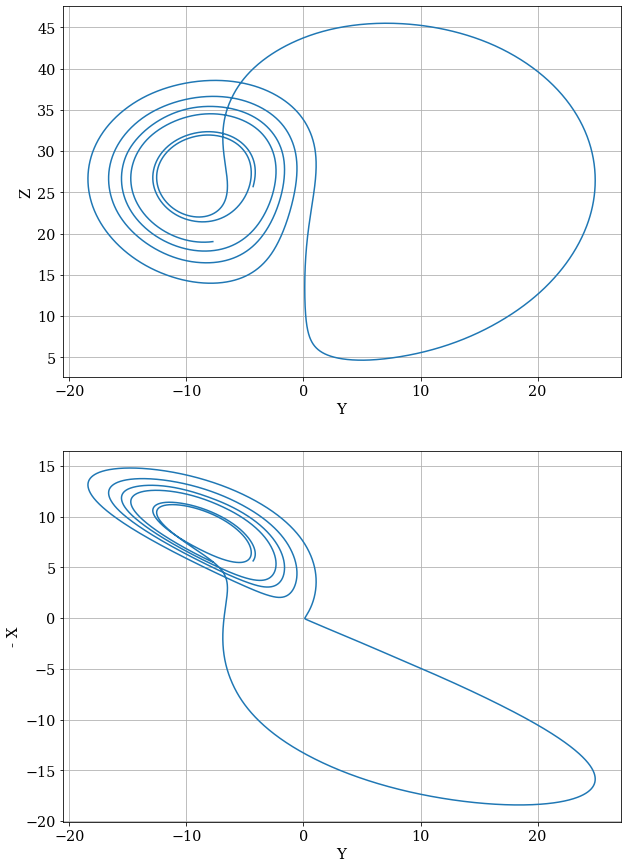
\includegraphics[width = 0.4\textwidth, height = 0.35\textwidth]{q2fig2.png}\label{fig:q2fig1B}}
    \hfill
  \caption{Recreated figures from \cite{Lorenz}. \label{fig:q2}}
\end{figure}
Figure \ref{fig:q2fig1a} displays the solution to equation \ref{eq:x} over $0\le t \le10$ (top), the solution to equation \ref{eq:y} over $10\le t \le 20$ (middle) and the solution to equation \ref{eq:z} over $20\le t \le30$ (bottom). The solution to equations \ref{eq:x}, \ref{eq:y} \& \ref{eq:z} were then computed over the time interval $14\le t \le 19$, these solutions on the Y-Z plane are shown in Figure \ref{fig:q2fig1B} (top) and solutions on the Y-X plane are shown in Figure \ref{fig:q2fig1B} (bottom). 

Next, the solution of equations \ref{eq:x}, \ref{eq:y} \& \ref{eq:z}, were computed with the initial condition $W_0' = W_0 + [0.0, 1.0\mathrm{e}{-8}, 0.0] = [0.0, 1.00000001, 0.0]$. The difference is defined by $W'-W$ such that $W'$ is the set of solutions with initial condition $W_0'$ and $W$ is the set of solutions with initial condition $W_0$. Figure \ref{fig:err_plts} displays the distance as a function of time on a semilog plot. The error is represented by an approximately linear line, this result agrees with the Lorenz's findings which is stated to indicate exponential growth.

\begin{figure}[H]
    \centering
    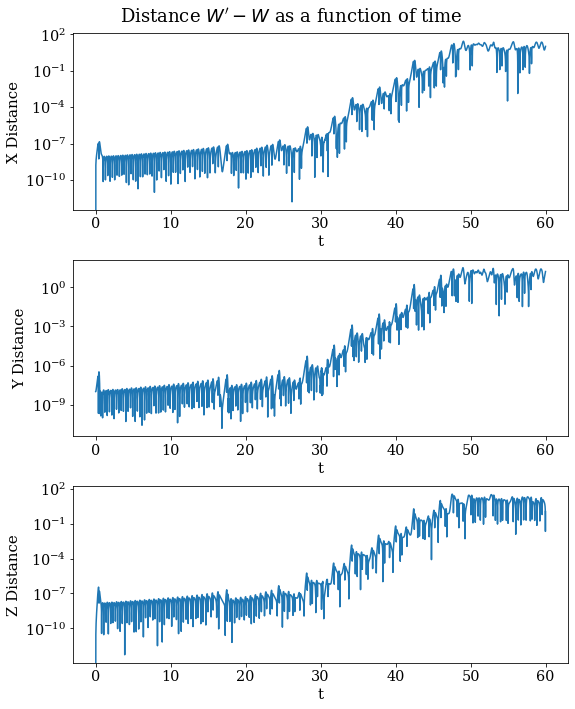
\includegraphics[width = 0.5\textwidth]{q2fig3.png}
    \caption{Distance $W'-W$ as a function of time.}
    \label{fig:err_plts}
\end{figure}

\bibliography{bib}

\end{document}